\documentclass[11pt,a4paper]{article}
\usepackage[margin=1in]{geometry}
\usepackage{graphicx}
\usepackage{booktabs}
\usepackage{hyperref}
\usepackage{enumitem}
\usepackage{amsmath}
\graphicspath{{../figures/}}

\title{MLOps Report: IMDb Sentiment Analysis Pipeline}
\author{UPC MLOps Team}
\date{\today}

\begin{document}

\maketitle

\section{Introduction}
This report summarises the development of an end-to-end machine learning (ML) component for IMDb film review sentiment classification. The objective is to deliver a reproducible pipeline that ingests raw reviews, trains a text classifier, and exposes evaluation artefacts suitable for integration into a broader ML-based product. The project embraces MLOps practices, including data versioning, configuration management, and automated evaluation.

\section{Dataset Overview}
The pipeline sources the public \texttt{imdb} dataset from Hugging Face via the \texttt{datasets} library (\texttt{mlops\_imdb/data/download\_imdb.py}). The dataset consists of 50{,}000 English-language movie reviews labelled as positive (\(1\)) or negative (\(0\)), already split into equally sized training and test partitions. After download, raw files are stored under \texttt{data/raw/} for reproducibility.

\section{Exploratory Data Analysis}
Preliminary exploration, performed in \texttt{notebooks/1.0-exploration-imdb.ipynb}, guides feature design and model assumptions. The balanced label split helps ensure unbiased optimisation (Figure~\ref{fig:label_dist}), while the long-tailed review length distribution (Figure~\ref{fig:text_len}) motivated normalising whitespace and retaining bi-grams during TF--IDF feature extraction.

\begin{figure}[h]
  \centering
  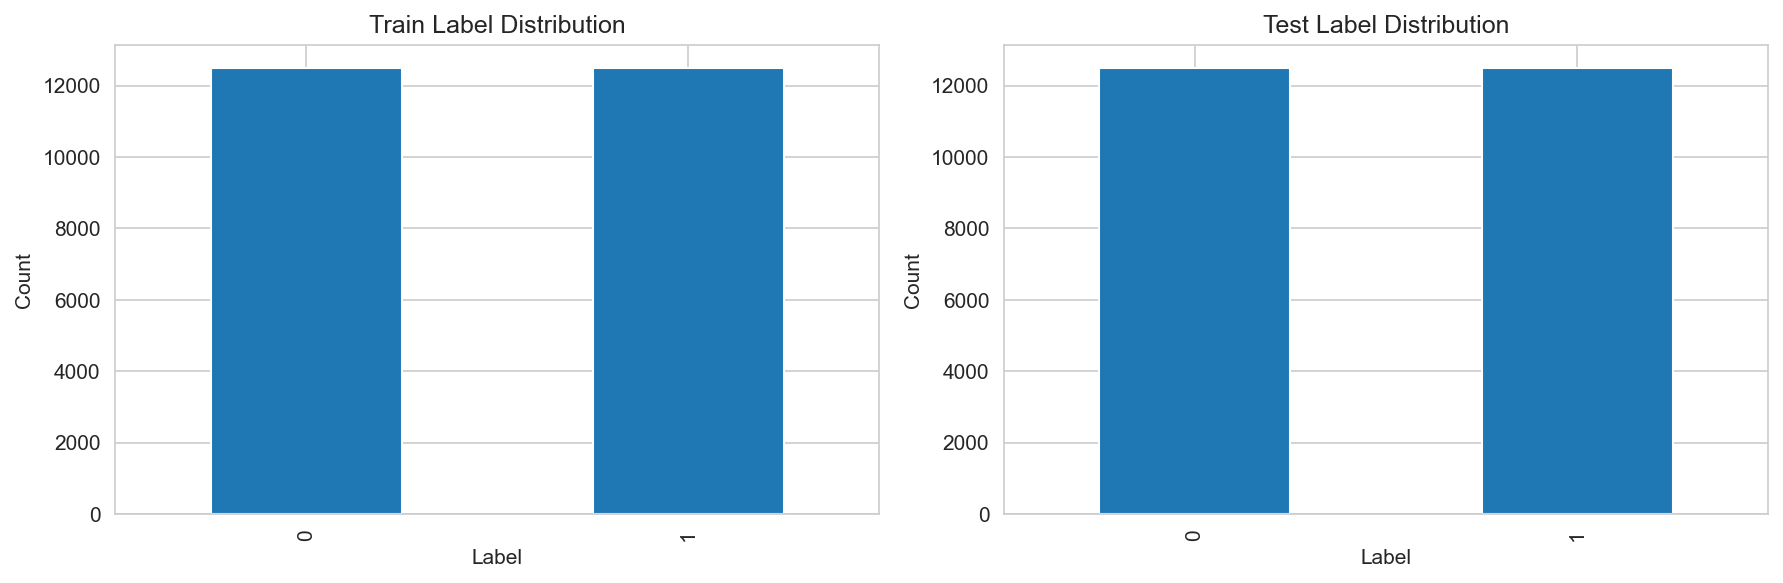
\includegraphics[width=1\textwidth]{label_distribution.png}
  \caption{Sentiment label distribution in the IMDb dataset (train + test).}
  \label{fig:label_dist}
\end{figure}

\begin{figure}[h]
  \centering
  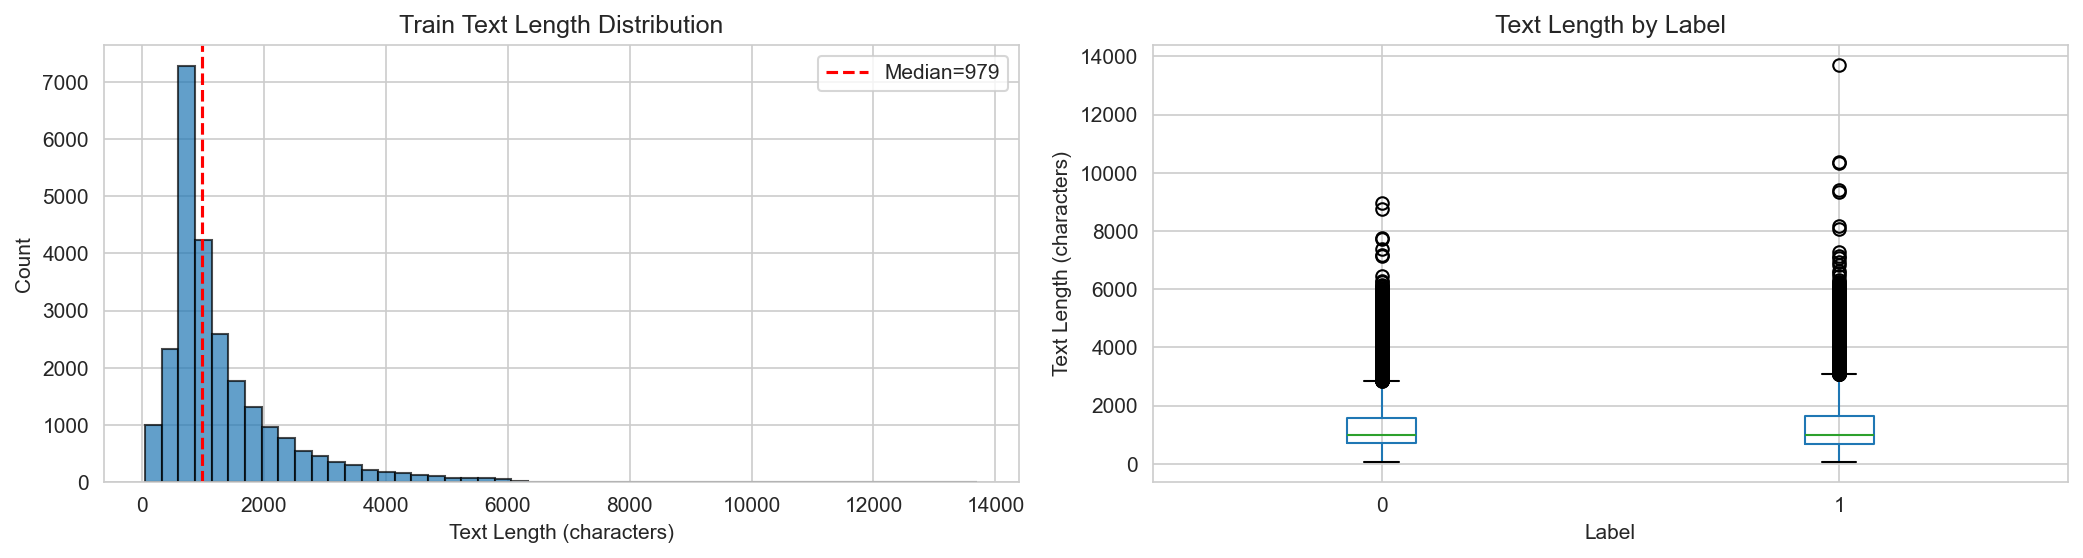
\includegraphics[width=1\textwidth]{text_length_distribution.png}
  \caption{Distribution of tokenised review lengths highlighting long-form texts.}
  \label{fig:text_len}
\end{figure}

\section{Pipeline Orchestration and Tooling}
\begin{itemize}[leftmargin=*]
  \item \textbf{Pipeline management:} DVC orchestrates the stages defined in \texttt{dvc.yaml} (\texttt{prepare} \(\rightarrow\) \texttt{features} \(\rightarrow\) \texttt{train} \(\rightarrow\) \texttt{eval}). Parameterisation is centralised in \texttt{params.yaml}, enabling consistent configuration across stages.
  \item \textbf{Energy tracking:} Each stage optionally instantiates a CodeCarbon \texttt{EmissionsTracker}, configured via the \texttt{energy.codecarbon} section of \texttt{params.yaml}, to capture environmental impact.
  \item \textbf{Testing:} Pytest suites (e.g. \texttt{tests/data/test\_download\_imdb.py}) validate critical behaviours such as dataset retrieval, safeguarding the pipeline against regressions.
\end{itemize}

\section{Data Preparation}
The preparation step (\texttt{mlops\_imdb/data/prepare.py}) performs deterministic cleansing:
\begin{itemize}[leftmargin=*]
  \item Lowercases text and removes HTML tags.
  \item Decodes HTML entities and normalises whitespace, ensuring compact token sequences.
  \item Validates required schema columns (\texttt{text}, \texttt{label}) in both train and test CSVs.
\end{itemize}
The cleaned outputs are saved to \texttt{data/processed/train\_clean.csv} and \texttt{data/processed/test\_clean.csv}. A fixed random seed (\(42\)) is maintained for any stochastic operations, although the current pipeline leverages the canonical IMDb split.

\section{Feature Engineering}
TF--IDF features are produced in \texttt{mlops\_imdb/features/build\_features.py}. Key configuration values include:
\begin{itemize}[leftmargin=*]
  \item Maximum vocabulary size of 10{,}000 terms.
  \item Bi-gram coverage via \(n\)-gram range \([1, 2]\).
  \item Frequency cut-offs with \texttt{min\_df} \(=2\) and \texttt{max\_df} \(=0.95\).
\end{itemize}
The resulting sparse matrices are persisted as \texttt{.npz} files for both training and test sets, alongside the serialised \texttt{TfidfVectorizer}. This design minimises memory footprint and keeps model training decoupled from textual pre-processing.

\section{Model Training}
A logistic regression classifier (\texttt{mlops\_imdb/modeling/train.py}) is trained on the TF--IDF features. The configuration leverages the \texttt{liblinear} solver to handle sparse input efficiently, with \( \texttt{max\_iter} = 1000 \) and \( \texttt{random\_state} = 42 \). The fitted model is persisted to \texttt{models/model.pkl} using \texttt{joblib}, ensuring compatibility with downstream inference scripts such as \texttt{mlops\_imdb/modeling/predict\_one.py}.

\section{Model Evaluation}
The evaluation stage (\texttt{mlops\_imdb/modeling/eval.py}) loads the trained model and test features to compute standard classification metrics. Results are stored in \texttt{reports/metrics.json} and a confusion matrix figure (\texttt{reports/figures/baseline\_confusion\_matrix.png}). Table~\ref{tab:metrics} summarises the latest evaluation run based on that artefact.

\begin{table}[h]
  \centering
  \caption{Binary classification performance on the IMDb test split.}
  \label{tab:metrics}
  \begin{tabular}{lcccc}
    \toprule
    Metric & Accuracy & Precision & Recall & F1-score \\
    \midrule
    Value & 0.8943 & 0.8907 & 0.8990 & 0.8948 \\
    \bottomrule
  \end{tabular}
\end{table}

The confusion matrix recorded in \texttt{reports/metrics.json} indicates balanced performance across classes:
\[
\begin{bmatrix}
11121 & 1379 \\
1263 & 11237
\end{bmatrix}
\]
which corresponds to 22{,}358 correct predictions out of 25{,}000 test samples. The model makes 1{,}379 false positives and 1{,}263 false negatives, highlighting slightly better recall than precision. Figure~\ref{fig:cm} illustrates the confusion matrix generated during evaluation.

\begin{figure}[h]
  \centering
  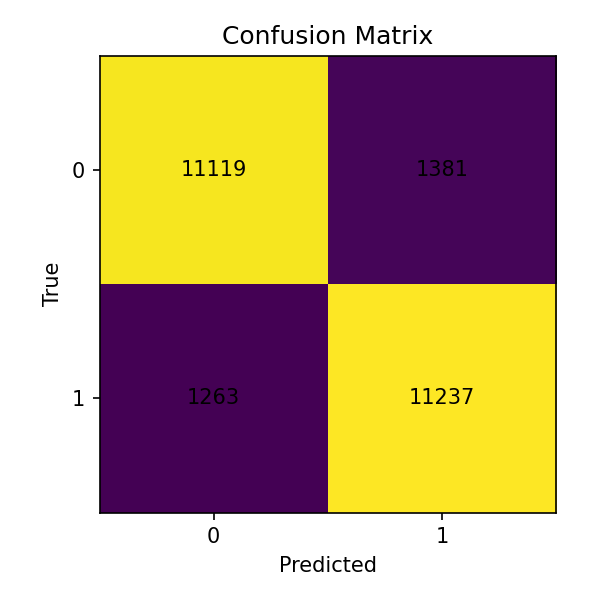
\includegraphics[width=0.8\textwidth]{baseline_confusion_matrix.png}
  \caption{Confusion matrix for the logistic regression classifier.}
  \label{fig:cm}
\end{figure}

QA thresholds specified in \texttt{params.yaml} (\( \texttt{min\_accuracy} = \texttt{min\_f1} = 0.85 \)) are satisfied, supporting promotion of this model to downstream environments.

\section{Energy and Carbon Monitoring}
DVC runs executed with CodeCarbon tracking (\texttt{reports/codecarbon\_emissions.csv}) show that the full pipeline emitted only \(7.15\)~mg CO\(_2\)eq over \(27.1\)~seconds on the Apple~M4 development laptop. Table~\ref{tab:carbon} details the per-stage footprint, highlighting feature extraction as the dominant contributor. Power traces stored in \texttt{reports/powermetrics\_log.txt} confirm modest CPU draw (approximately \(3.4\)~W) with no GPU utilisation, consistent with the lightweight logistic-regression workload.

\begin{table}[h]
  \centering
  \caption{CodeCarbon emissions per pipeline stage (values in mg CO\(_2\)eq).}
  \label{tab:carbon}
  \begin{tabular}{lcc}
    \toprule
    Stage & Duration (s) & Emissions (mg) \\
    \midrule
    Prepare data & 5.51 & 1.21 \\
    Build features & 14.46 & 5.52 \\
    Train model & 3.47 & 0.21 \\
    Evaluate model & 3.63 & 0.22 \\
    \midrule
    \textbf{Total} & 27.07 & \textbf{7.15} \\
    \bottomrule
  \end{tabular}
\end{table}

\section{Coding Standards and Tooling}
Static analysis relies on Ruff, configured in \texttt{pyproject.toml} to enforce a project-wide line length of \(99\) characters and to treat \texttt{mlops\_imdb} as the first-party import namespace. The configuration enables both linting and auto-formatting, with import ordering (\texttt{I} checks) turned on so that \texttt{ruff check} harmonises third-party and local imports. These conventions are codified in the Make targets \texttt{make lint} (audit only) and \texttt{make format} (auto-fix then format). The \texttt{dev} dependency group also pins Ruff for local development and integrates with optional pre-commit hooks, ensuring contributors receive consistent feedback before code reaches the repository.

\section{Operational Considerations}
\begin{itemize}[leftmargin=*]
  \item \textbf{Reproducibility:} DVC pipelines combined with version-controlled parameters guarantee deterministic runs. Processed artefacts (cleaned data, features, model, metrics) are stored under tracked directories, simplifying handoffs.
  \item \textbf{Deployment readiness:} The project includes inference scripts (\texttt{mlops\_imdb/modeling/predict\_one.py}) and configurable prediction paths (\texttt{params.yaml}) to facilitate batch or online scoring workflows.
  \item \textbf{Energy monitoring:} CodeCarbon hooks produce emissions reports (e.g. \texttt{reports/codecarbon\_emissions.csv}), enabling sustainability tracking for future iterations.
\end{itemize}

\section{MLflow Tracking (Placeholder)}
MLflow integration is planned but not yet implemented. This section will outline experiment tracking configuration, run metadata, and metric logging once the team enables MLflow in the pipeline.

\section{Conclusions and Next Steps}
The current pipeline delivers a robust baseline sentiment model with near 90\% accuracy on IMDb reviews. Immediate next steps include:
\begin{itemize}[leftmargin=*]
  \item Integrating MLflow to manage experiment metadata and model registry operations.
  \item Evaluating alternative models (e.g. linear SVM, transformer-based encoders) to benchmark gains over logistic regression.
  \item Expanding automated tests to cover feature generation and evaluation logic, further strengthening quality assurance.
\end{itemize}

\end{document}
